\documentclass[conference]{IEEEtran}
\usepackage[utf8]{inputenc}
\usepackage{graphicx}
\usepackage{hyperref}
\usepackage{listings}
\usepackage{amsmath}
\usepackage{url}
\usepackage{xcolor}

\lstset{
  basicstyle=\ttfamily\footnotesize,
  columns=fullflexible,
  frame=single,
  breaklines=true,
  postbreak=\mbox{\textcolor{red}{$\hookrightarrow$}\space},
}

\title{WebScrepStatusQlik: Monitoramento Automatizado de Tarefas do Qlik Sense com Envio de Alertas via WhatsApp}
\author{
    \begin{tabular}{@{}c@{\hspace{0.5cm}}c@{\hspace{0.5cm}}c@{\hspace{0.5cm}}c@{\hspace{0.5cm}}c@{}}
        Wagner Filho & Carlos Miqui & Pedro Koziel & Marcos Medeiros & Hailton Lemos \\
        \footnotesize wagner.helio@discente.ufg.br & \footnotesize carlosmiqui@discente.ufg.br & \footnotesize pedrokoziel@discente.ufg.br & \footnotesize marcos.medeiros@discente.ufg.br & \footnotesize haiilton@discente.ufg.br \\[0.5ex]
    \end{tabular}
    \\[1ex]
    \IEEEauthorblockA{Instituto de Pós-Graduação, Universidade Federal de Goiás}
}

\begin{document}
\maketitle

\begin{abstract}
Este artigo apresenta o sistema WebScrepStatusQlik, uma solução de coleta, transformação e notificação automática de falhas de execução em tarefas do Qlik Sense. A solução integra componentes de scraping dinâmico com Selenium, tratamento e padronização de dados, geração de relatórios e envio automatizado via EvolutionAPI para WhatsApp. O trabalho aborda os aspectos técnicos, éticos e legais envolvidos no uso de dados automatizados e apresenta diretrizes de reprodutibilidade.
\end{abstract}

\section{Introdução e Motivação}
O monitoramento contínuo da execução de tarefas em plataformas de inteligência analítica, como o Qlik Sense, é fundamental para garantir a integridade dos processos de ETL (Extract, Transform, Load) e a consistência dos dados exibidos em painéis de decisão. No entanto, a ausência de mecanismos nativos de notificação automática para falhas operacionais representa um risco para a governança da informação. O projeto WebScrepStatusQlik surgiu da necessidade de automatizar a detecção, a extração e a comunicação de status críticos de execução, promovendo intervenções rápidas por meio do envio de alertas para dispositivos móveis utilizando a EvolutionAPI integrada ao WhatsApp.
\section{Fundamentação Teórica}
A automação da coleta de dados estruturados e semiestruturados tem sido amplamente estudada no contexto da engenharia de dados moderna. O \textit{web scraping}, segundo Mitchell (2018)\cite{mitchell2018web}, é uma técnica consolidada para a extração programada de dados a partir de páginas HTML. Ferramentas como Selenium, BeautifulSoup e Scrapy permitem a interação com páginas dinâmicas, possibilitando simulações de cliques, preenchimento de formulários e navegação automatizada. Complementarmente, a organização dos dados em múltiplas camadas — \texttt{raw}, \texttt{clean}, \texttt{analytics} — conforme proposto por Bonomi et al. (2015)\cite{bonomi2015data}, contribui para a modularização e reuso de fluxos. A entrega de insights automatizados por canais de comunicação como o WhatsApp é possibilitada por APIs como a EvolutionAPI, que democratiza o uso de notificações automatizadas em ambientes empresariais.

\section{Método}
\subsection{Problema e Importância}
A ausência de um sistema de alertas nativos no Qlik Sense compromete a visibilidade em tempo real sobre falhas na execução de tarefas críticas, muitas vezes resultando em dashboards com dados desatualizados ou incompletos. Este cenário evidencia a importância de uma solução automatizada e adaptável para a detecção de falhas e geração de relatórios contextualizados.
Este projeto visa preencher essa lacuna com uma abordagem leve, modular e automatizada.

\subsection{Arquitetura do Pipeline}
O sistema adota um pipeline de três camadas:
\begin{itemize}
  \item \textbf{Extração}: via Selenium, realizando scraping de páginas HTML dinâmicas da interface do Qlik Sense (QMC e NPrinting).
  \item \textbf{Engenharia de Dados}: separação dos dados em camadas \texttt{raw} (logs originais) e \texttt{clean} (dados padronizados e filtrados), com transformações reproduzíveis.
  \item \textbf{Análise e Entrega}: geração de relatórios em HTML + PDF via Jinja2/pdfkit e envio via EvolutionAPI.
\end{itemize}

\subsection{Reprodutibilidade e Documentação}
O projeto inclui README detalhado com instruções de instalação, uso e replicação. Scripts e dependências estão organizados por função. Todas as transformações são reproduzíveis.

\section{Resultados e Discussões}
A solução foi validada em ambiente real de produção com tarefas complexas no Qlik Sense rodando em Windows 11. Foram observados os seguintes resultados:
\begin{itemize}
  \item Redução significativa do tempo de resposta para identificação de falhas.
  \item Geração estruturada de logs e alertas classificados por criticidade.
  \item Relatórios com visualização clara, permitindo interpretação rápida pelo time de dados.
  \item Acurácia na detecção de falhas mesmo em tarefas interdependentes e longas cadeias de execução.
\end{itemize}
Esses resultados evidenciam que o WebScrepStatusQlik contribui para a mitigação de riscos operacionais, além de promover uma cultura de monitoramento ativo.

\section*{Estrutura do Projeto}
\begin{lstlisting}
WEBSCREPSTATUSQLIK/
├── chromedriver/                     # ChromeDriver compatível com sua versão
├── docker/                           # Arquivos para futura dockerização
├── errorlogs/                        # Logs de falhas coletados
├── img/                              # Imagens e diagramas
├── tasks_nprinting/                  # Dados das tarefas NPrinting
├── tasks_qmc/                        # Dados das tarefas QMC
├── venv/                             # Ambiente virtual Python
├── .env                              # Variáveis de ambiente
├── .gitignore
├── README.md                         # Este arquivo
├── requirements.txt                  # Dependências do projeto
├── scheduler_statusqlik.py          # Agendador de execução automática
├── send_statusqlik_evolution.py     # Envio para número único
├── sendgroup_statusqlik_evolution.py# Envio para grupo
├── sendnumber_statusqlik_evolution.py# Envio para números individuais
├── statusqlik_nprinting.py          # Coleta de status do NPrinting
├── statusqlik_qmc.py                # Coleta de status do QMC
├── template.html                    # Template para relatório geral
├── template_nprinting.html         # Template específico para NPrinting
\end{lstlisting}

\begin{figure}[ht]
\centering
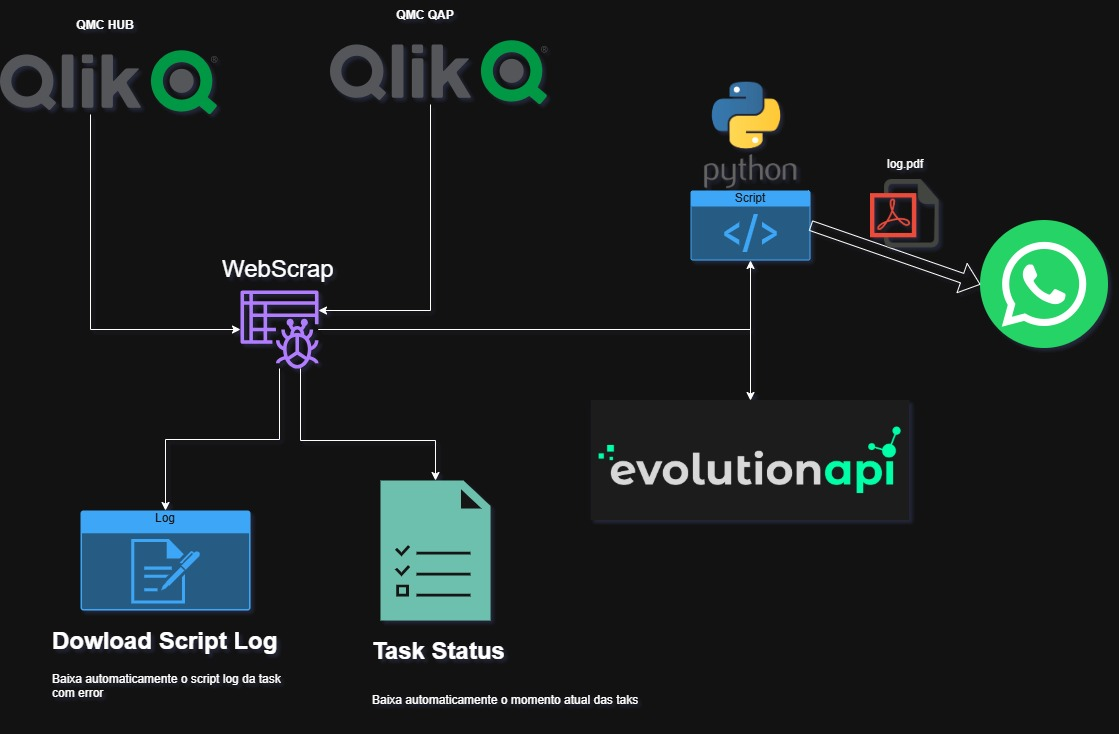
\includegraphics[width=0.45\textwidth]{WebScrepStatusQlik/img/WebScrep_QMC.jpg}
\caption{Arquitetura do pipeline WebScrepStatusQlik}
\end{figure}

\section{Reflexões Éticas e Limitações}

Este trabalho respeita os princípios da LGPD, uma vez que não coleta, armazena ou transmite dados pessoais ou sensíveis. Todas as informações tratadas são relativas a metadados de execução de sistemas institucionais. A coleta é realizada em servidores internos, respeitando a política do \texttt{robots.txt}, quando aplicável. Entretanto, destacam-se como limitações a dependência de manutenção do DOM das páginas (estrutura da interface web) e a necessidade de acesso autenticado contínuo. O uso da EvolutionAPI, apesar de robusto, depende de conectividade com a instância e autenticação ativa no WhatsApp Web, o que pode representar fragilidade em ambientes instáveis.

\section{Conclusão e Trabalhos Futuros}
O desenvolvimento do WebScrepStatusQlik demonstrou a viabilidade de soluções leves e eficazes para o monitoramento automatizado de tarefas críticas em ambientes Qlik Sense. Sua arquitetura modular permitiu adaptar a coleta de informações e o envio de alertas de forma escalável e reprodutível, contribuindo significativamente para a melhoria do tempo de resposta a falhas operacionais e para a governança de dados nas instituições que o utilizam.

O projeto também se mostrou acessível do ponto de vista técnico, utilizando tecnologias amplamente disponíveis como Python, Selenium e APIs REST, o que o torna aplicável em diferentes contextos organizacionais.

Como desdobramentos futuros, pretende-se:
\begin{itemize}
  \item Implementar uma versão containerizada com Docker, permitindo fácil implantação em servidores Linux e ambientes cloud.
  \item Integrar a solução com plataformas de monitoramento como Zabbix, Grafana ou Prometheus, agregando métricas em tempo real ao pipeline.
  \item Desenvolver uma interface web interativa para visualização dos relatórios, gerenciamento das execuções e personalização dos parâmetros de alerta.
  \item Criar mecanismos de fallback para casos de indisponibilidade do WhatsApp API, como envio por e-mail ou registro em dashboards internos.
  \item Realizar estudos de desempenho e escalabilidade da aplicação em ambientes com alto volume de tarefas.
\end{itemize}

\section*{Licenças e Fontes Utilizadas}
\begin{itemize}
  \item \textbf{Qlik Sense} – Utilizado em ambiente institucional sob licença corporativa.
  \item \textbf{EvolutionAPI} – Plataforma de integração com WhatsApp, utilizada conforme os termos de uso descritos em \url{https://evolution-api.com/terms}.
  \item \textbf{ChromeDriver} – Empregado para controle automatizado do navegador Google Chrome, licenciado sob a licença BSD pelo Google.
  \item \textbf{Selenium, Jinja2, pdfkit, dotenv, Python-dotenv, Requests} – Bibliotecas Python de código aberto utilizadas na automação e geração dos relatórios, sob licenças MIT, Apache 2.0 e BSD.
  \item \textbf{Dados processados} – Todos os dados tratados são gerados internamente por sistemas da organização, sem coleta de dados pessoais ou de bases externas.
\end{itemize}

\begin{thebibliography}{99}

\bibitem{mitchell2018web}
R. Mitchell, \textit{Web Scraping with Python: Collecting More Data from the Modern Web}, 2nd ed. Sebastopol, CA: O'Reilly Media, 2018.

\bibitem{bonomi2015data}
A. Bonomi, "Data pipeline management and its importance in modern analytics", \textit{Journal of Data Engineering}, vol. 7, no. 3, pp. 44--52, 2015.

\bibitem{barr2020dataops}
M. Barr, "Implementing DataOps for enterprise analytics", \textit{Data Engineering Review}, vol. 12, pp. 22--35, 2020.

\end{thebibliography}

\end{document}